\subsection{Auswertung}
Um das laufende Training oder bereits abgeschlossene Trainings zu bewerten oder vergleichen nutzt Unity ML-Agents Tensorboard. Tensorboard visualisiert die Metriken des Trainings in Zeitgraphen (siehe Abbildung \ref{fig:tensorboard}). Der wichtigste Graph ist die gesammelte Belohnung. Für Implementierungen mit \hl{frühem Stoppen} ist die erreichte Episodenlänge auch sehr Aussage kräftig. Unter der Rubrik Policy finden sich auch die Graphen welche den Verlauf der Hyperparameter darstellen. Die linke Seitenleiste listet alle im aktuellen Verzeichnis gespeicherten Trainings auf. Darüber können Trainingsets ausgewählt und anschließend in den Graphen durch unterschiedlich farbige Linien verglichen werden.

\begin{figure}[H]
  \centering  
  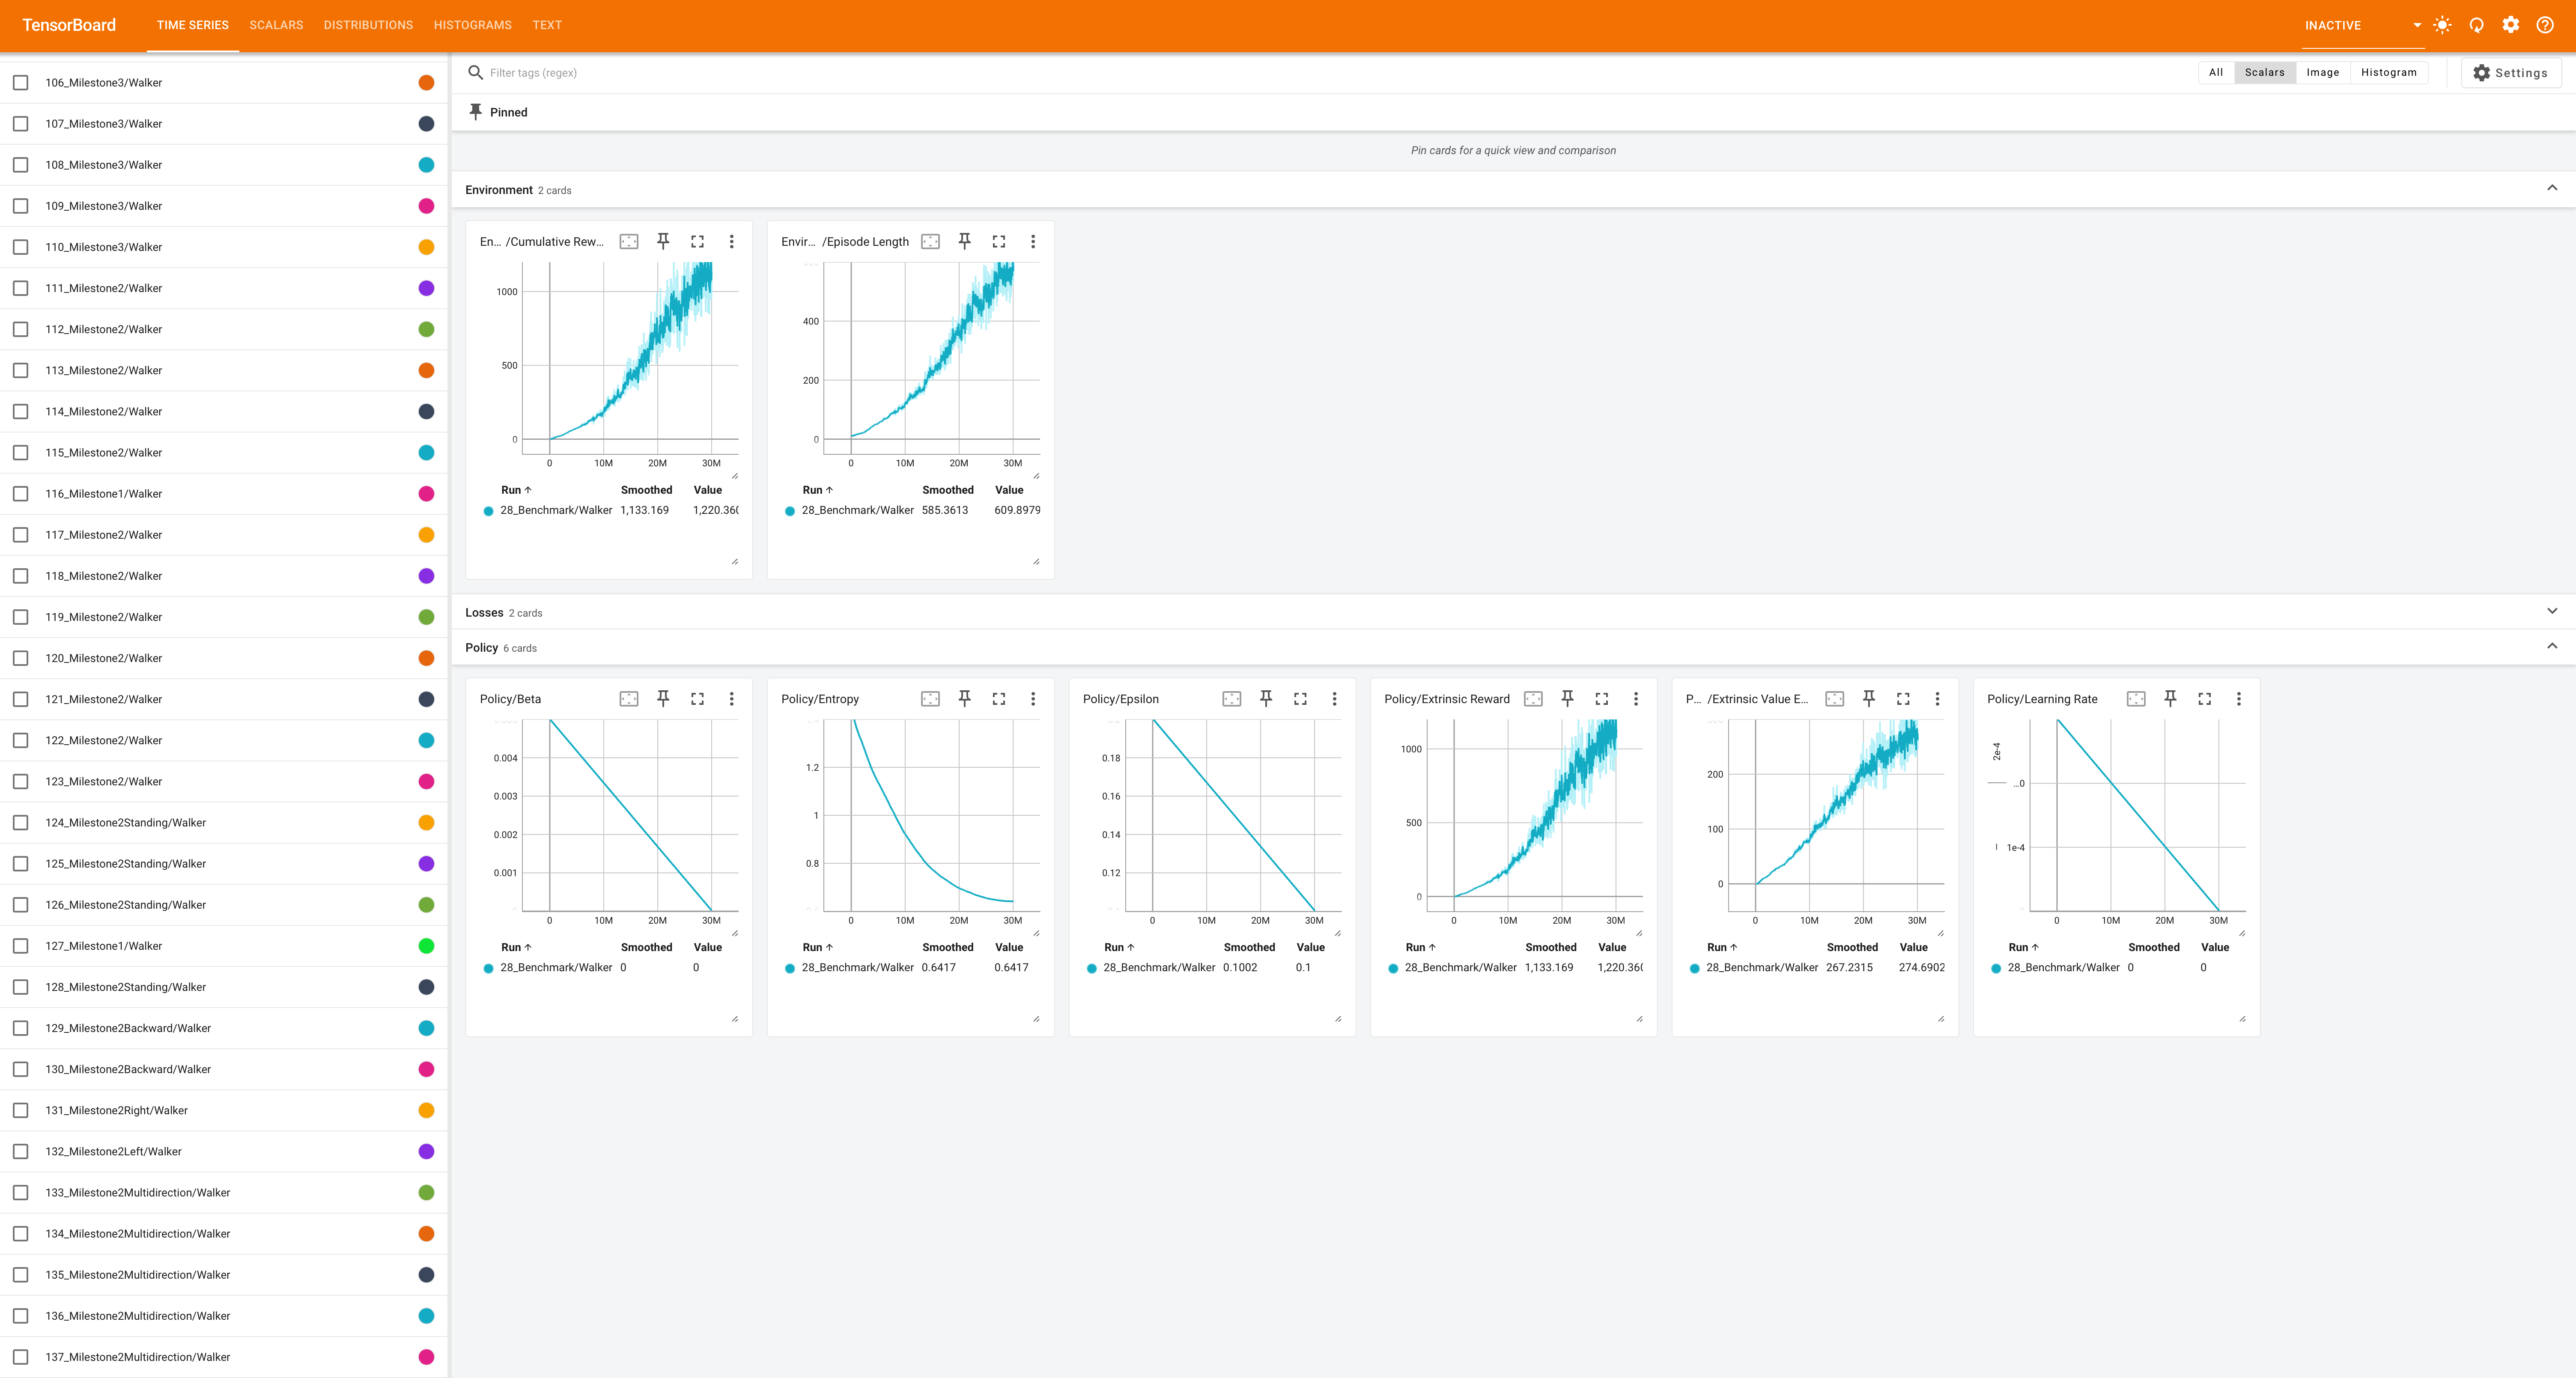
\includegraphics[scale=0.15]{img/tensorboard.png}
  \caption{Tensorboard Ansicht}
  \label{fig:tensorboard}
\end{figure}

Nicht immer geben die vorgefertigten Graphen alle relevanten Informationen wieder. Um die erfassten Daten und damit die Graphen zu erweitern bietet Unity ML-Agents über die Statistikrekorder die Statistik Hinzufügen Funktion. Neu hinzugefügte Werte werden über die Episode und alle Umgebungen aggregiert. Als Aggregationsmethode kann zwischen Duchschnitt und letzter Wert entschieden werden. In Tensorboard werden die neuen Statistiken anschließen dargestellt.

Die letzte Instanz der Auswertung ist das Abspielen des trainierten Modells in der Unity Umgebung. In den meisten Fällen ist die grafische Darstellung das zuverlässigste Medium um das trainierte Modell zu bewerten.